\documentclass[border=10pt]{standalone}
\usepackage{pgfplots}
\pgfplotsset{compat=1.18}
\begin{document}
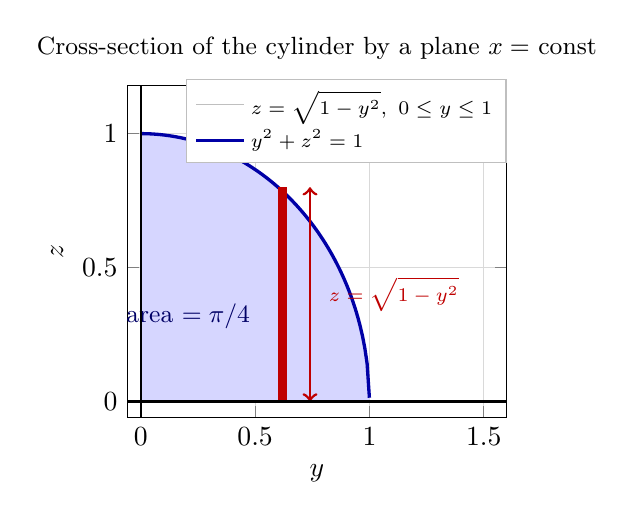
\begin{tikzpicture}
\begin{axis}[
    width=6.4cm, height=5.8cm,
    xmin=-0.06, xmax=1.60, ymin=-0.06, ymax=1.18,
    xlabel=$y$, ylabel=$z$,
    grid=major, grid style={black!15},
    title={Cross-section of the cylinder by a plane $x=$ const},
    title style={font=\small},
    legend style={at={(1.0,1.02)}, anchor=north east, font=\scriptsize,
                  fill=white, draw=black!25, cells={anchor=west}}]
    \addplot[fill=blue!16, draw=none, domain=0:1, samples=100] {sqrt(1-x^2)} \closedcycle;
    \addlegendentry{$z=\sqrt{1-y^{2}},\ 0\le y\le 1$}
    \addplot[blue!65!black, line width=1.2pt, domain=0:1, samples=100] {sqrt(1-x^2)};
    \addlegendentry{$y^{2}+z^{2}=1$}
    \addplot[fill=red!75!black, draw=none] coordinates {(0.60,0) (0.64,0) (0.64,0.80) (0.60,0.80)};
    \draw[red!75!black, line width=1pt, <->] (axis cs:0.74,0) -- (axis cs:0.74,0.80);
    \node[font=\scriptsize, text=red!75!black, anchor=west] at (axis cs:0.78,0.40) {$z=\sqrt{1-y^{2}}$};
    \node[font=\small, text=blue!40!black, anchor=north east] at (axis cs:0.52,0.40)
        {area $=\pi/4$};
    \draw[black, line width=0.8pt] (axis cs:-0.06,0) -- (axis cs:1.60,0);
    \draw[black, line width=0.8pt] (axis cs:0,-0.06) -- (axis cs:0,1.18);
\end{axis}
\end{tikzpicture}
\end{document}
